\mode*
\section{Integration}
\subsection{Einführung}

%\mmode<article>{
Wir beginnen die Einführung des Integrals mit einem Beispiel aus dem täglichen Leben. In der Schule lernt man den Ausdruck \glqq{}Strecke ist Zeit mal Geschwindigkeit\grqq{}. Dies gilt aber nur für konstante Geschwindigkeit. Hier schauen wir uns diesen Sachverhalt im Detail an und entwickeln daraus ein neues Konzept.
%}

%%%%%%%%%%%%%%%%%%%%%%%%%%%%%%%%%%%%%%%%%%%%%%%%%%%%%%%%%%%%
\begin{frame}{Beispiel: Strecke als Integral der Geschwindigkeit}
    \begin{itemize}
        \item Wir befinden uns in einem Auto oder auf einem Fahrrad
        \item Zu jedem Zeitpunkt sieht man auf dem Geschwindigkeitsmesser die Geschwindigkeit $v$ in $\nicefrac{km}{h}$
        \item Welche Strecke $s$ legen wir in einem Zeitintervall $\Delta t$ zwischen 1 und 3 Stunden nach Fahrtbeginn zurück?
        \item Dazu modellieren wir die Geschwindigkeit zum jeweiligen Zeitpunkt $t$ als Funktionswert $v(t)$
    \end{itemize}
\end{frame}

%%%%%%%%%%%%%%%%%%%%%%%%%%%%%%%%%%%%%%%%%%%%%%%%%%%%%%%%%%%%
\begin{frame}
    \frametitle<presentation>{Konstante Geschwindigkeit}
    Wir beginnen mit dem einfachen Beispiel einer Fahrt mit konstanter Geschwindigkeit:
    \begin{itemize}
        \item<+-> Frage: welche Strecke $s$ legen wir im Zeitintervall zwischen 1 und 3 Stunden nach Fahrtbeginn bei konstanter Geschwindigkeit $v=20 \nicefrac{km}{h}$ zurück?
        \item<+-> Wir erhalten $s=\Delta t \cdot v$, also
        $s=2h \cdot 20\frac{km}{h}=40km$
        \item<+-> Die Strecke entspricht der Fläche des Rechtecks in der Grafik
    \begin{center}
        \includegraphics[width=.6\textwidth]{fig/integral0}
    \end{center}
    \end{itemize}    
\end{frame}

Ist die Geschwindigkeit variabel, so müssen wir das Konzept erweitern. Wie wir am folgenden Bild einer Geschwindigkeitskurve sehen, können wir nicht wie vorher einfach ein Rechteck zeichnen. Statt des einfachen Produkts der Geschwindigkeit mit der Zeit führen wir einen neuen mathematischen Begriff ein, das \textit{Integral}. Im Folgenden überlegen wir dann, wie wir diesen Begriff so definieren, dass er einerseits der Intuition des täglichen Lebens genügt, andererseits aber mathematisch präzise genug ist, um ihn zuverlässig verwenden zu können.
%%%%%%%%%%%%%%%%%%%%%%%%%%%%%%%%%%%%%%%%%%%%%%%%%%%%%%%%%%%%
\begin{frame}
    \frametitle<presentation>{Variable Geschwindigkeit}
        \begin{center}
        \includegraphics[width=.6\textwidth]{fig/integral-kurve}
    \end{center}       

     Sprechweise: Die Strecke $s$ ist das \textbf{Integral} der Geschwindigkeit $v$ über das Zeitintervall $(t_0,t_1)$.
     In mathematischer Notation
     \begin{gather*}
         s = \int_{t_0}^{t_1} v(t) \, dt.
     \end{gather*}
\end{frame}

Wir versuchen uns nun dem Integral anzunähern, indem wir es von unten und oben einschließen. Dazu bestimmen wir die minimale und maximale Geschwindigkeit.
%%%%%%%%%%%%%%%%%%%%%%%%%%%%%%%%%%%%%%%%%%%%%%%%%%%%%%%%%%%%
\begin{frame}
    \frametitle<presentation>{Variable Geschwindigkeit -- erste Näherung}
    \begin{center}
        \includegraphics[width=.45\textwidth]{fig/integral1}
    \end{center}
    \mode<presentation>{\only<1>{\begin{Denkpause}
        Wir wollen das Integral durch Einschließung annähern. Können Sie aus dem Bild Ober- und Untergrenzen schließen?
    \end{Denkpause}}}
    \pause
Das Integral liegt zwischen den Strecken, die wir bei konstanter Minimal- bzw. Maximalgeschwindigkeit gefahren wären:
\begin{gather*}
    {\color{red}v_{\text{min}} \Delta t}
    \le \int_{t_0}^{t_1} v(t) \,dt
    \le {\color{blue}v_{\text{max}} \Delta t}
\end{gather*}
\end{frame}

Das ist offensichtlich eine sehr grobe Abschätzung. Wir können sie aber verbessern, wenn wir kleinere Intervalle nehmen.
%%%%%%%%%%%%%%%%%%%%%%%%%%%%%%%%%%%%%%%%%%%%%%%%%%%%%%%%%%%%
\begin{frame}
    \frametitle<presentation>{Variable Geschwindigkeit -- Teilung der Intervalle}
    \begin{center}
        \includegraphics[width=.45\textwidth]{fig/integral2}
        \includegraphics[width=.45\textwidth]{fig/integral4}
    \end{center}
 \begin{itemize}
    \item Wir teilen das Zeitintervall in Teilintervalle und addieren die Ergebnisse
    \begin{gather*}
    \hspace*{-6mm}
    {\color{red}
        \sum_{i=1}^{2} v^{(i)}_{\text{min}} \tfrac{\Delta t}{2}
        \le \sum_{i=1}^{4} v^{(i)}_{\text{min}} \tfrac{\Delta t}{4}
    }
    \le \int_{t_0}^{t_1} v(t) \,dt
    \le {\color{blue}
        \sum_{i=1}^{4} v^{(i)}_{\text{max}} \tfrac{\Delta t}{4}
        \le \sum_{i=1}^{2} v^{(i)}_{\text{max}} \tfrac{\Delta t}{2}
    }        
    \end{gather*}
     \item Intuitiv bekommen wir genauere Ergebnisse
 \end{itemize}
\end{frame}

%%%%%%%%%%%%%%%%%%%%%%%%%%%%%%%%%%%%%%%%%%%%%%%%%%%%%%%%%%%%
\begin{frame}
    \frametitle<presentation>{Sukzessive Intervallteilung}
\begin{center}
    \begin{minipage}[t]{.43\textwidth}
    \vspace*{0mm}
    \includegraphics[width=\textwidth]{fig/integral1}
    \end{minipage}
    \begin{minipage}[t]{.43\textwidth}
    \vspace*{0mm}
    \includegraphics[width=\textwidth]{fig/integral2}
    \end{minipage}

    \begin{minipage}[t]{.43\textwidth}
    \vspace*{0mm}
    \includegraphics[width=\textwidth]{fig/integral4}
    \end{minipage}
    \begin{minipage}[t]{.43\textwidth}
    \vspace*{0mm}
    \includegraphics[width=\textwidth]{fig/integral8}
    \end{minipage}
\end{center}
\end{frame}
Die Bilder zeigen exemplarisch, wie sich die Maxima und Minima immer mehr dem Graphen der Funktion annähern. Auch sehen wir, wie die Fläche des blauen Bereichs, die gerade die Differenz zwischen Unter- und Obersumme darstellt, schrumpft.

%%%%%%%%%%%%%%%%%%%%%%%%%%%%%%%%%%%%%%%%%%%%%%%%%%%%%%%%%%%%
\begin{frame}{Das Integral als Grenzwert}
\begin{itemize}
    \item<+-> Setzen wir den Prozess der Intervallhalbierung fort, so sehen wir:
    \begin{itemize}
        \item Die Summen der Minima (Untersummen) bilden eine monoton wachsende Folge
        \item Die Summen der Maxima (Obersummen) bilden eine monoton fallende Folge
        \item Es gilt
        \begin{gather*}
                {\color{red}
        \sum_{i=1}^{2^n} v_{i,\text{min}} \tfrac{\Delta t}{2^n}
    }
    \le \int_{t_0}^{t_1} v(t) \,dt
    \le {\color{blue}
        \sum_{i=1}^{2^n} v_{i,\text{max}} \tfrac{\Delta t}{2^n}
    }        
        \end{gather*}
    \end{itemize}
        \item<+-> Daher konvergieren Unter- und Obersummen zu Grenzwerten ${\color{red}S_*}$ und ${\color{blue}S^*}$ mit
        \begin{gather*}
            {\color{red}S_*} \le \int_{t_0}^{t_1} v(t) \,dt
            \le {\color{blue}S^*}.
        \end{gather*}
        \item<+-> Sind beide Grenzwerte gleich, so ist das Integral eindeutig bestimmt
\end{itemize}
\end{frame}

\begin{Wdh}
    Sollten Sie sich nicht erinnern, warum monotone, beschränkte Folgen konvergieren, ist das eine gute Gelegenheit, den Abschnitt aus dem Vorsemester nachzulesen.
\end{Wdh}

%%%%%%%%%%%%%%%%%%%%%%%%%%%%%%%%%%%%%%%%%%%%%%%%%%%%%%%%%%%%
\begin{frame}{Das Integral als Fläche unter einer Kurve}
    \begin{itemize}
        \item Die stückweise konstanten Funktionen, die die Unter- und Obersummen definieren, konvergieren gegen die Funktion $v$.
        \begin{itemize}
            \item ...zumindest, wenn $v$ stetig ist.
        \end{itemize}
        \item Wir schließen, dass das Integral die Fläche zwischen der Funktion $v$ und der $t$-Achse beschreibt
        \item Die Einheit der Fläche ist das Produkt der Einheiten der horizontalen und vertikalen Achsen
        \item<2-> Ist die Funktion negativ, so ist das Integral negativ
        \begin{itemize}
            \item Das Integral ist die Fläche mit Vorzeichen!
        \end{itemize}
    \end{itemize}
\end{frame}

%%%%%%%%%%%%%%%%%%%%%%%%%%%%%%%%%%%%%%%%%%%%%%%%%%%%%%%%%%%%
\begin{Vertiefung}
    Die Unter- und Obersummen haben die allgemeine Form
    \begin{gather*}
        S_n = \sum_{i=1}^n f_i h_i,\qquad h_i = x_i-x_{i-1},
    \end{gather*}
    wobei das Intervall $[a,b]$ durch die Punkte
    \begin{gather*}
        a = x_0 < x_1 < \dots < x_n = b
    \end{gather*}
    in $n$ Teilintervalle geteilt wird. $f_i$ ist ein Funktionswert auf dem Teilintervall $[x_{i-1},x_i]$.
    Die $h_i$ nennen wir Gewichte, da sie angeben, wie groß der Anteil von $f_i$ an der Summe ist. Für die Gewichte $h_i$ gilt unabhängig von $n$ 
    \begin{gather*}
        \sum_{i=1}^n h_i = b-a.
    \end{gather*}
Wir nennen Summen dieser Art Riemannsche Summen.    
Hier haben wir uns von Zweierpotenzen als Intervallzahlen und auch von dem Zwang gelöst, dass alle Intervalle gleich lang sein müssen. Stattdessen kann $n$ nun eine beliebige Zahl sein, und für den Grenzprozess denken wir natürlich an eine Folge in der $n$ gegen unendlich geht.
Umso wichtiger ist die Tatsache, dass die Summe aller Gewichte $h_i$ von $n$ unabhängig ist. Daraus folgt dann zum Beispiel sofort, dass die Riemannschen Summen beschränkt bleiben, wenn die Funktion $f$ beschränkt ist.

Was wir durch diese Verallgemeinerung verlieren, ist die Monotonie der Folgen der Unter- und Obersummen. Stattdessen müssen gegebenenfalls andere Konvergenzkriterien herangezogen werden. Lassen Sie uns aber nicht vergessen, dass diese Argumente nur zur Herleitung des Integralbegriffs benötigt werden, nicht zur Berechnung von Integralen.

Bei einer sauberen, mathematischen Definition muss man noch sicherstellen, dass die Grenzwerte der Ober- und Untersummen nicht von der Wahl der einzelnen Intervalle abhängen, solange alle Intervalllängen gegen null konvergieren. Das ist in der Tat aufwändiger als es für diesen Kurs angemessen ist.

Historisch haben sich zwei Integralbegriffe durchgesetzt, die nach ihren Entdeckern Riemann und Lebesgue benannt sind. Wenn beide Integrale existieren, haben sie denselben Wert, weshalb die Unterscheidung für uns irrelevant ist.
Für die Anwendung ist wesentlich, dass nach Lebesgue praktisch jede Funktion integrierbar ist, also dies nie zusätzlich als Voraussetzung gefordert werden muss. Das Riemann-Integral ist zwar mit weniger mathematischem Aufwand definierbar, doch ist dort der Test, ob eine Funktion integrierbar ist, kompliziert.

Wir überlassen diese Details gern den Mathematikern und benutzen die Integrale im Vertrauen auf deren Arbeit. Insbesondere nehmen wir an, dass jede Funktion, die für uns relevant ist, auch integrierbar ist, und fordern das im Folgenden nicht mehr explizit.
\end{Vertiefung}

\begin{frame}{Integrierbarkeit}
    In vielen mathematischen Texten wird die \textbf{Integrierbarkeit} von Funktionen diskutiert, meist im Kontext des Riemann-Integrals. Das ist mathematisch abwegig und für Anwendungen irrelevant.

    \pause

    \begin{block}{Für uns als Anwender gilt:}
        Jede beschränkte Funktion ist integrierbar.
    \end{block}
\end{frame}

\begin{frame}{Beispiel im Plenum}
    Für einen Punkt $x>0$ werden wir das Integral
    \begin{gather*}
        \int_0^x t^2\,dt
    \end{gather*}
    berechnen, indem wir für $n$ Teilintervalle der Länge $\Delta t = \nicefrac xn$ die Unter- und Obersummen berechnen und den Grenzwert für $n\to\infty$ untersuchen.
\end{frame}

%\mmode<article>{
\begin{Aufgabe}
  Ziel dieser Aufgabe ist es, für einen Punkt $x$ das Integral
  \begin{gather*}
      \int_0^x t\,dt
  \end{gather*}
  über den beschriebenen Näherungsprozess zu berechnen. Teilen Sie dazu das Intervall $[0,x]$ in $n$ Teilintervalle der Länge $\Delta t = \nicefrac{x}{n}$.
  \begin{enumerate}
      \item Schreiben Sie für festes $n$ die Ober- und Untersummen.
      \item Überführen Sie sie in eine Form, die in den Summen kein $x$ mehr enthält.
      \item Wenden Sie die Summenformeln aus dem ersten Semester oder aus dem Internet an
      \item Betrachten Sie nun die Ergebnisse im Grenzwert $n\to\infty$.
      \begin{enumerate}
          \item Bestimmen Sie die Grenzwerte $(n-1)\Delta t$, $n\Delta t$, und $(n+1)\Delta t$.
          \item Bestimmen Sie den Grenzwert der Summenformeln
      \end{enumerate}
      \item Ist das Integral eindeutig bestimmt?
      \item (Denkaufgabe ohne Bewertung) Können Sie sich einen Ersatz für Unter- und Obersummen denken, der das Integral wesentlich besser approximiert?
  \end{enumerate}
\end{Aufgabe}
%}

\begin{frame}{Abschlussfragen}
    \begin{enumerate}
        \item Für welche Objekte können wir die Flächen elementar berechnen?
        \item Was ist der mathematische Begriff für die Fläche unter/über einer Funktion?
        \item Wie kann diese Fläche angenähert werden?
        \item Wie ist sie definiert?
    \end{enumerate}
\end{frame}

%%%%%%%%%%%%%%%%%%%%%%%%%%%%%%%%%%%%%%%%%%%%%%%%%%%%%%%%%%%%
%%%%%%%%%%%%%%%%%%%%%%%%%%%%%%%%%%%%%%%%%%%%%%%%%%%%%%%%%%%%
\subsection{Rechnen mit Integralen}
%%%%%%%%%%%%%%%%%%%%%%%%%%%%%%%%%%%%%%%%%%%%%%%%%%%%%%%%%%%%
\begin{frame}{Schreib- und Sprechweise}
Notation des Integrals
    \begin{gather*}
        \int_a^b f(t)\,dt
    \end{gather*}
    \begin{itemize}
        \item $a$ und $b$ sind die \textbf{untere} und \textbf{obere Integrationsgrenze}
        \item Das Intervall $[a,b]$ ist der \textbf{Integrationsbereich}
        \item die Funktion $f$ ist der \textbf{Integrand}
        \item $dt$ ist das \textbf{Differenzial}
        \item $t$, die Variable im Differenzial, ist die \textbf{Integrationsvariable}
    \end{itemize}
\end{frame}

%%%%%%%%%%%%%%%%%%%%%%%%%%%%%%%%%%%%%%%%%%%%%%%%%%%%%%%%%%%%
\begin{frame}{Integrationsvariable}
    \begin{itemize}
        \item die Integrationsvariable kann beliebig gewählt werden
        \begin{gather*}
            \int_a^bf(t)\,dt = \int_a^b f(x)\,dx = \int_a^b f(y)\,dy
        \end{gather*}
        \item die Integrationsvariable darf allerdings nicht identisch zu einer Integrationsgrenze sein, also
        \begin{gather*}
            \int_0^x f(t)\,dt
            \quad\text{ist erlaubt,}\quad
            \int_0^x f(x)\,dx
            \quad\text{ist nicht erlaubt.}
        \end{gather*}
    \end{itemize}
\end{frame}

%%%%%%%%%%%%%%%%%%%%%%%%%%%%%%%%%%%%%%%%%%%%%%%%%%%%%%%%%%%%
\begin{frame}{Vertauschung der Integralgrenzen}
  Aus der Herleitung des Integrals folgt für die Vertauschung der Integrationsgrenzen
  \begin{gather*}
      \int_a^b f(t)\,dt = - \int _b^a f(t)\,dt
  \end{gather*}
  Insbesondere gilt damit für jede Funktion $f$
  \begin{gather*}
      \int_a^a f(t)\,dt = 0.
  \end{gather*}
  Daraus wiederum folgt, dass wir den Wert einer Funktion in einzelnen Punkten beliebig ändern dürfen, ohne den Wert des Integrals zu ändern. Das gilt sogar für abzählbar viele Punkte.
\end{frame}

%%%%%%%%%%%%%%%%%%%%%%%%%%%%%%%%%%%%%%%%%%%%%%%%%%%%%%%%%%%%
\begin{frame}{Integrationsbereiche}
  Das Integral ist \glqq{}additiv\grqq{} bezüglich der Integrationsintervalle
  \begin{gather*}
      \int_a^b f(t)\,dt = \int_a^c f(t)\,dt + \int_c^b f(t)\,dt
  \end{gather*}
  Das gilt das auch, wenn $c$ nicht zwischen $a$ und $b$ liegt.
\end{frame}

%%%%%%%%%%%%%%%%%%%%%%%%%%%%%%%%%%%%%%%%%%%%%%%%%%%%%%%%%%%%
\begin{frame}{Monotonie}
    Für alle $t$ aus dem Intervall $[a,b]$ gelte $f(t) \le g(t)$. Dann gilt
    \begin{gather*}
        \int_a^b f(t)\,dt \le \int_a^b g(t)\,dt.
    \end{gather*}
    \pause
    Insbesondere gilt dann: wenn $f(t) \ge 0$ auf $[a,b]$, dann gilt
    \begin{gather*}
        \int_a^b f(t)\,dt \ge 0.
    \end{gather*}
\end{frame}

%%%%%%%%%%%%%%%%%%%%%%%%%%%%%%%%%%%%%%%%%%%%%%%%%%%%%%%%%%%%
\begin{frame}{Arithmetik mit Integralen}
    Integrale sind Summen, daher hat Multiplikation als Operator Vorrang und die Klammern hier sind optional:
    \begin{gather*}
        \int_a^b \bigl(f(t)g(t)\bigr)\,dt = \int_a^b f(t)g(t)\,dt
    \end{gather*}
    Summen von Integralen mit identischen Integrationsintervallen können vereinigt oder getrennt werden. Beachten Sie, dass links geklammert werden muss:
    \begin{gather*}
        \int_a^b \bigl(f(t)+g(t)\bigr)\,dt
        =
        \int_a^b f(t)\,dt + \int_a^b g(t)\,dt
    \end{gather*}
    Konstante Faktoren darf man \glqq{}herausziehen\grqq{}:
    \begin{gather*}
        \int_a^b \lambda f(t)\,dt = \lambda\int_a^b f(t)\,dt
    \end{gather*}
\end{frame}

%%%%%%%%%%%%%%%%%%%%%%%%%%%%%%%%%%%%%%%%%%%%%%%%%%%%%%%%%%%%
\begin{frame}{Gerade und ungerade Funktionen}
\mode<article>{Wenn Funktionen symmetrisch zum Mittelpunkt des Integrationsintervals  sind, vereinfacht sich die Integration. Sind sie achsensymmetrisch spricht man von geraden Funktionen, sind sie punktsymmetrisch von ungeraden. Insbesondere im letzten Fall ist das Integral null, man spart sich also komplett das rechnen.}
    \begin{columns}
        \begin{column}{.5\textwidth}
        \begin{block}{Gerade Funktion}
            \begin{gather*}
                f(-x) = f(x)
            \end{gather*}
            \resizebox{\columnwidth}{!}{\begin{tikzpicture}%[x=1cm,y=0.6cm]

% ---------- Parameter (einheitliche Boxgrößen) ----------
\def\xmin{-3.5}
\def\xmax{ 3.5}

% Für die TRIG-Zeile: einheitlicher y-Bereich
\def\yminTrig{-1.5}
\def\ymaxTrig{ 1.5}

% Gesamt-Boundingbox festlegen (wichtig für Resizebox/Columns und damit nichts "überlappt")
%\useasboundingbox (\xmin,\yminTrig) rectangle (\xmax,\ymaxPoly+\rowsep);

% ===================
% unten: cos(x) (gerade → blau)
% ===================
\begin{scope}
  \clip (\xmin,\yminTrig) rectangle (\xmax,\ymaxTrig);

  \draw[->] (\xmin,0) -- (\xmax,0);
  \draw[->] (0,\yminTrig) -- (0,\ymaxTrig);

  \draw[domain=\xmin:\xmax, samples=200, smooth, thick, blue]
    plot ({\x},{cos(\x r)});

  % Symmetrie-Markierung (±1)
  \draw[dashed] (1,0) -- (1,{cos(1 r)});
  \draw[dashed] (-1,0) -- (-1,{cos(1 r)});
  \filldraw[blue] (1,{cos(1 r)}) circle (2pt);
  \filldraw[blue] (-1,{cos(1 r)}) circle (2pt);
\end{scope}

\end{tikzpicture}}
            \begin{gather*}
                \int_{-a}^a f(t)\,dt = 2\int_0^a f(t)\,dt
            \end{gather*}
        \end{block}
    \end{column}
    \begin{column}{.5\textwidth}
        \begin{block}{Ungerade Funktion}
            \begin{gather*}
                f(-x) = -f(x)
            \end{gather*}
            \resizebox{\columnwidth}{!}{\begin{tikzpicture}%[x=1cm,y=0.6cm]

% ---------- Parameter (einheitliche Boxgrößen) ----------
\def\xmin{-3.5}
\def\xmax{ 3.5}

% Für die TRIG-Zeile
\def\yminTrig{-1.5}
\def\ymaxTrig{ 1.5}

\def\rowsep{8.2}

% Gesamt-Boundingbox festlegen
%\useasboundingbox (\xmin,\yminTrig) rectangle (\xmax,\ymaxPoly+\rowsep);

% ===================
% unten: sin(x) (ungerade → rot)
% ===================
\begin{scope}
  \clip (\xmin,\yminTrig) rectangle (\xmax,\ymaxTrig);

  \draw[->] (\xmin,0) -- (\xmax,0);
  \draw[->] (0,\yminTrig) -- (0,\ymaxTrig);

  \draw[domain=\xmin:\xmax, samples=200, smooth, thick, red]
    plot ({\x},{sin(\x r)});

  % Ursprungssymmetrie-Markierung
  \filldraw[red] (0,0) circle (2pt);
  \filldraw[red] (1,{sin(1 r)}) circle (2pt);
  \filldraw[red] (-1,{-sin(1 r)}) circle (2pt);
\end{scope}

\end{tikzpicture}}
            \begin{gather*}
                \int_{-a}^a f(t)\,dt = 0
            \end{gather*}
        \end{block}
    \end{column}
    \end{columns}
    
    Anmerkung: natürlich kann man den Begriff gerade/ungerade auch bezüglich eines anderen Mittelpunktes definieren
\end{frame}

%%%%%%%%%%%%%%%%%%%%%%%%%%%%%%%%%%%%%%%%%%%%%%%%%%%%%%%%%%%%
\begin{frame}{Definition: Mittelwert}
    Sei $f$ eine Funktion auf $[a,b]$. Die Zahl
    \begin{gather*}
        m = \frac{1}{b-a} \int_a^b f(t)\,dt
    \end{gather*}
    heißt \textbf{Mittelwert} von $f$ auf dem Intervall $[a,b]$. Sie ist der Wert der konstanten Funktion, die über das Intervall $(a,b)$ dasselbe Integral wie $f$ hat.
\end{frame}
%%%%%%%%%%%%%%%%%%%%%%%%%%%%%%%%%%%%%%%%%%%%%%%%%%%%%%%%%%%%
\begin{frame}{Mittelwertsatz}
        %\includegraphics[width=.45\textwidth]{fig/Mittelwertsatz} funktioniert nicht so ganz
        \begin{itemize}
            \item Gegeben sei eine beliebige stetige Funktion $f$ auf einem Intervall $[a,b]$
            \item<+-> Dann gibt es stets ein $z\in(a,b)$, so dass
            \begin{gather*}
                \int_a^b f(t)\, dt = f(z)(b-a)
            \end{gather*}
        \end{itemize}
\end{frame}

%%%%%%%%%%%%%%%%%%%%%%%%%%%%%%%%%%%%%%%%%%%%%%%%%%%%%%%%%%%%
\begin{frame}{Bestimmtes und unbestimmtes Integral}
    Integrale mit fest bestimmten Integralgrenzen, z.B.
    \begin{gather*}
        \int_a^bf(t) \,dt, \qquad \int_1^3f(t)\,dt
    \end{gather*}
    \begin{itemize} 
        \item bezeichnet man als \textbf{bestimmte Integrale}
        \item $a$ und $b$ sind hier fest vorgegebene Zahlen
        \item Ausgehend von einer \textit{Funktion} erhält man eine \textit{Zahl}
    \end{itemize}
    \pause
    Integrale, bei denen nur eine Grenze bestimmt ist, die andere aber eine Variable
    \begin{gather*}
        F(x) \equiv \int_a^x f(t) dt, \qquad\qquad F(x) \equiv \int_0^x f(t)dt
    \end{gather*}
    \begin{itemize} 
        \item bezeichnet man als \textbf{unbestimmte Integrale}.
        \item Durch Variation von $x$ erhält man verschiedene \textit{reelle Zahlen}. Dies kann als neue Funktion $F(x)$ interpretiert werden.
    \end{itemize}
\end{frame}



%%%%%%%%%%%%%%%%%%%%%%%%%%%%%%%%%%%%%%%%%%%%%%%%%%%%%%%%%%%%
\begin{frame}{\glqq{}Hauptsatz\grqq{} der Differential- und Integralrechnung}
    Sei $f$ eine stetige Funktion und $F$ das unbestimmte Integral definiert durch 
    \begin{gather*}
        F(x) = \int_a^x f(t)\,dt.
    \end{gather*}
    \begin{columns}
        \begin{column}{.59\textwidth}
        Es gilt dann für Differenzen benachbarter Punkte
        \begin{align*}
            F(x\!+\!h)\!-\!F(x) &= 
            \int^{{\color{blue}x+h}}_{\color{red}a} f(t)\,dt -\! {\color{red}\int_a^x} f(t)\,dt
            \\&= {\color{blue}\int_x^{x+h}} f(t)\,dt
            \\&= h f(z)
        \end{align*}
        wobei wir den Mittelwertsatz angewandt haben.
        \end{column}
        \begin{column}{.39\textwidth}
            \begin{flushright}
            \includegraphics[width=.8\textwidth]{fig/integral-hauptsatz.tikz}
            \end{flushright}
        \end{column}
    \end{columns}
\end{frame}

Nun teilen wir durch $h$ und lassen $h$ gegen null konvergieren. Es gilt dann
\begin{gather*}
    \lim_{h\to 0}\frac{F(x+h)-F(x)}{h}
    = \lim_{h\to 0} f(z) = f(x),
\end{gather*}
wobei wir benutzt haben, dass für beliebiges $h$ der Punkt $z$ zwischen $x$ und $x+h$ liegt und daher $z\to x$ konvergiert.
Wir gelangen somit zum sogenannten Hauptsatz der Differential- und Integralrechnung: 
%%%%%%%%%%%%%%%%%%%%%%%%%%%%%%%%%%%%%%%%%%%%%%%%%%%%%%%%%%%%
\begin{frame}
    \frametitle<presentation>{\glqq{}Hauptsatz\grqq{} der Differential- und Integralrechnung}
Sei $f$ eine stetige Funktion und $F$ das unbestimmte Integral
\begin{gather*}
    F(x) = \int_{a}^x f(t)\,dt.
\end{gather*}
Dann ist $F$ stetig differenzierbar und es gilt
    \begin{gather*}
        F'(x) = \frac{d}{dx} \int_{a}^x f(t)\,dt = f(x).
    \end{gather*}
\end{frame}

%%%%%%%%%%%%%%%%%%%%%%%%%%%%%%%%%%%%%%%%%%%%%%%%%%%%%%%%%%%%
\begin{frame}{Stammfunktion}
     Eine \textbf{Stammfunktion} $F$ einer Funktion $f$ ist eine Funktion $F$, so dass gilt:
     \begin{gather*}
         F' = f.
     \end{gather*}
 
    \begin{itemize}
    \item<+-> Eine Stammfunktion ist nur bis auf eine Konstante bestimmt, ansonsten ist sie eindeutig. Schreibweise: $F(x)+C$
    \item<+-> Das unbestimmte Integral
    \begin{gather*}
        U(x) = \int_a^x f(t)\,dt
    \end{gather*}
    ist nach dem Hauptsatz eine Stammfunktion von $f$ und es gilt $U(a) = 0$
    \item<+-> Für beliebige Intervalle $[a,b]$ im Definitionsbereich von $f$ und eine beliebige Stammfunktion $F$ gilt:
     \begin{gather*}
         U(b) = \int_a^b f(t)\,dt = F(b)-F(a).
     \end{gather*}
     \end{itemize}
\end{frame}

\begin{frame}{Abschlussfragen}
\begin{enumerate}
    \item Warum kann es praktisch sein zu betrachten, ob eine Funktion gerade bzw. ungerade ist?
    \item Was erhalten Sie, wenn Sie eine Stammfunktion der Funktion $f$ ableiten?
    \item Was erhalten Sie, wenn Sie $F$ ableiten und die Stammfunktion der Ableitung bilden?
    \item Wie hilft die Stammfunktion bei der Bestimmung unbestimmter und bestimmter Integrale?
\end{enumerate}    
\end{frame}

%%%%%%%%%%%%%%%%%%%%%%%%%%%%%%%%%%%%%%%%%%%%%%%%%%%%%%%%%%%%
%%%%%%%%%%%%%%%%%%%%%%%%%%%%%%%%%%%%%%%%%%%%%%%%%%%%%%%%%%%%
\subsection{Berechnung von Integralen}
%%%%%%%%%%%%%%%%%%%%%%%%%%%%%%%%%%%%%%%%%%%%%%%%%%%%%%%%%%%%
\begin{frame}{Berechnung mit Hilfe der Stammfunktion}

    Für die Stammfunktion gilt $F'(x) = f(x)$. Daraus ergibt sich der folgende
    \begin{block}{Algorithmus}
        \begin{enumerate}
        \item Finde zu $f$ eine Stammfunktion $F$.
        \item Wende die Formel für das Integral an.
     \begin{gather*}
         \int_a^b f(t)\,dt = F(b)-F(a).
     \end{gather*}
    \end{enumerate}
    \end{block}
\end{frame}

%%%%%%%%%%%%%%%%%%%%%%%%%%%%%%%%%%%%%%%%%%%%%%%%%%%%%%%%%%%%
\begin{frame}{Beispiele}
    \begin{gather*}
        f(x) = x,\quad f(x) = x^2, \quad f(x) = x^n
    \end{gather*}
    \pause
    \begin{gather*}
        \frac1{x^2},\quad \frac1{x^3},\quad \frac1{x^n}
    \end{gather*}
    \pause
    \begin{block}{Stammfunktion von Potenzen von $x$}
    \begin{gather*}
        f(x) = x^n,
        \qquad
        F(x) = \tfrac1{n+1}x^{n+1}
    \end{gather*}
    für $n\neq -1$.
    \end{block}
\end{frame}

%%%%%%%%%%%%%%%%%%%%%%%%%%%%%%%%%%%%%%%%%%%%%%%%%%%%%%%%%%%%
\begin{frame}{Grundlegende Technik}
    Raten und Überprüfung durch Ableitung
    \begin{align*}
        \sin'(x) &= \cos(x)\\
        \cos'(x) &= -\sin(x)\\
        \tfrac{d}{dx} e^x &= e^x\\
        \tfrac{d}{dx} \ln \left|x\right| &= \tfrac1x
    \end{align*}
\end{frame}

%%%%%%%%%%%%%%%%%%%%%%%%%%%%%%%%%%%%%%%%%%%%%%%%%%%%%%%%%%%%
\begin{frame}{Partielle Integration}
    Erinnerung: Produktregel $(fg)' = f'g+fg'$ daher $f'g = (fg)'-fg'$
    \pause
    \begin{gather*}
        \int_a^b f'(t)g(t)\,dt = \Bigl[f(t)g(t)\Bigr]_a^b
        -\int_a^b f(t)g'(t)\,dt.
    \end{gather*}
    Kurzschreibweise: $\Bigl[u(t)\Bigr]_a^b = u(b)-u(a)$

    Anwendung: Man kann den Integranden als Produkt schreiben und kennt eine Stammfunktion für einen Faktor

    \pause
    Achtung: es wird keine Stammfunktion berechnet, sondern ein (un-)bestimmtes Integral!
\end{frame}

Ein Beispiel ist das Integral des Logarithmus. Nehmen wir an, dass $a>b>0$, dann gilt:
\begin{align*}
    \int_a^b \ln t\,dt
    &= \int_a^b 1\ln t\,dt\\
    &= \Bigl[ t\ln t\Bigr]_a^b - \int_a^b t\frac1t \,dt\\
    &= \Bigl[ t\ln t - t\Bigr]_a^b
\end{align*}
Darüber können wir jetzt sogar eine Stammfunktion als unbestimmtes Integral berechnen. Am einfachsten wäre das mit den Integrationsgrenzen 0 und $x$. Der Term $x\ln x$ konvergiert gegen 0 für $x\to 0$, daher existiert das uneigentliche Integral
\begin{gather*}
    \int_0^b \ln t\,dt = b \ln b - b,
\end{gather*}
und ersetzen wir nun die feste Grenze $b$ durch die Variable Grenze $x$, so erhalten wir zur Funktion $f(x) = \ln x$ die Stammfunktion
\begin{gather*}
    F(x) = x\ln x - x + C.
\end{gather*}

\begin{Aufgabe}
Berechnen Sie folgende Integrale mittels partieller Integration. \textit{Hinweis:} Sie müssen diese Methoden ggf. mehrfach anwenden.
    \begin{align*}
    \begin{alignedat}{3}
    \text{a)}\;& \int_0^{\ln{(2)}} xe^x\, dx \qquad &
    \text{b)}\;& \int  x \cos(x) \, dx \qquad &
    \text{c)}\;& \int  x^2e^x\,dx \qquad \\
    \text{d)}\;& \int_0^{\pi} x^2\sin(x)\,dx \qquad &
    \text{e)}\;& \int  \sin(x)\cos(x)\,dx \qquad
    \end{alignedat}
    \end{align*}
\end{Aufgabe}

%%%%%%%%%%%%%%%%%%%%%%%%%%%%%%%%%%%%%%%%%%%%%%%%%%%%%%%%%%%%
\begin{frame}{Lineare Substitution}
    \begin{gather*}
        \int_a^b f(\alpha t+\beta) \,dt
        = \frac1\alpha \int_{\alpha a+\beta}^{\alpha b+\beta} f(t)\,dt
    \end{gather*}

\begin{columns}
    \begin{column}{.49\textwidth}
        \begin{center}
            \includegraphics[width=.9\textwidth]{fig/integral-scale.tikz}
        \end{center}
        \begin{gather*}
            {\color{blue}\int_0^{a} f(2t)\,dt}
            =
            {\color{red}\int_0^{2a} f(t)\,dt}
        \end{gather*}
    \end{column}
    \begin{column}{.49\textwidth}
        \begin{center}
            \includegraphics[width=.9\textwidth]{fig/integral-shift.tikz}
        \end{center}
        \begin{gather*}
            {\color{blue}\int_0^{a} f(t+1)\,dt}
            =
            {\frac12\color{red}\int_1^{a+1} f(t)\,dt}
        \end{gather*}
    \end{column}
\end{columns}

\end{frame}

%%%%%%%%%%%%%%%%%%%%%%%%%%%%%%%%%%%%%%%%%%%%%%%%%%%%%%%%%%%%
\begin{frame}{Substitutionsregel 1. Form}
    Erinnerung: Kettenregel: $\tfrac{d}{dt} f\bigl(\phi(t)\bigr) = \phi'(t) f'\bigl(\phi(t)\bigr)$
    \pause
    \begin{block}{}
        Sei $x = \phi(t)$ und daher $\frac{dx}{dt} = \phi'(t)$ mit stetig differenzierbarem $\phi$. Dann gilt
        \begin{gather*}
            \int_a^b f\bigl(\phi(t)\bigr)\phi'(t)\,dt
            = \int_{\phi(a)}^{\phi(b)} f(x)\,dx.
        \end{gather*}
    \end{block}
    \pause
    Formal funktioniert die Substitutionsregel so, dass wir überall $\phi(t)$ durch $x$ ersetzen und formal
    \begin{gather*}
        dx = \frac{dx}{dt}\,dt = \phi'(t)\,dt
    \end{gather*}
    Die Integralgrenzen müssen nun auch in $x = \phi(t)$ ausgedrückt werden.
\end{frame}
%%%%%%%%%%%%%%%%%%%%%%%%%%%%%%%%%%%%%%%%%%%%%%%%%%%%%%%%%%%%
\begin{frame}{Beispiel}
    \begin{gather*}
        \int_a^b t \cos(t^2)\,dt
        \only<3->{=\frac12\int_{a^2}^{b^2} \cos(x)\,dx}
    \end{gather*}
    \pause
    Benutze $\phi(t) = t^2$, dann gilt $\phi'(t) = 2t$
\end{frame}

%%%%%%%%%%%%%%%%%%%%%%%%%%%%%%%%%%%%%%%%%%%%%%%%%%%%%%%%%%%%
\begin{frame}{Substitutionsregel 2. Form}
    \begin{block}{}
        Sei $x = \phi(t)$ und daher $\frac{dx}{dt} = \phi'(t)$ mit stetig differenzierbarer, \textbf{monotoner} Funktion $\phi$. Dann gilt
        \begin{gather*}
            \int_{a}^{b} f(x)\,dx =
            \int_{\phi^{-1}(a)}^{\phi^{-1}(b)} f\bigl(\phi(t)\bigr)\phi'(t)\,dt
            .
        \end{gather*}
    \end{block}
\end{frame}

Der Ausdruck $\phi^{-1}(x)$ bezeichnet hier die Umkehrfunktion zu $\phi(t)$. Deren Existenz ist es auch, die die Monotonie erfordert.

%%%%%%%%%%%%%%%%%%%%%%%%%%%%%%%%%%%%%%%%%%%%%%%%%%%%%%%%%%%%
\begin{frame}{Beispiel}
\label{frame:circle}
    Berechne das Integral
    \begin{gather*}
        \int_0^1 \sqrt{1-x^2}\,dx
    \end{gather*}
    \only<1>{\begin{Denkpause}
        Es sieht nicht so aus, als hätten wir hier eine wohlbekannte Ableitung als Faktor. Aber womit kann man die Wurzel vereinfachen?
    \end{Denkpause}}
    \pause
    Es gilt $1-\cos^2 t = \sin^2 t$, wodurch wir die Wurzel ziehen können. Also probieren wir die Substitution
    \begin{gather*}
        x = \cos t,\qquad dx = -\sin t \,dt.
    \end{gather*}
    \pause
    Berechnen wir zunächst die Stammfunktion:
    \begin{multline*}
        \int \sqrt{1-x^2}\,dx = - \int \sqrt{1-\cos^2 t}\sin t\,dt
        \\
        = -\int \sin^2 t\,dt
        = \frac{-1}2\int \bigl(1-\cos (2t)\bigr)\,dt
    \end{multline*}
\end{frame}

%%%%%%%%%%%%%%%%%%%%%%%%%%%%%%%%%%%%%%%%%%%%%%%%%%%%%%%%%%%%
\begin{frame}
    \frametitle<presentation>{Beispiel (Forts.)}
    Nun können wir elementar die Stammfunktion berechnen: 
    \begin{gather*}
        f(t) = \frac{\cos(2t)-1}{2},\qquad F(t) = \frac{-\sin(2t)}4-\frac t2
    \end{gather*}
    \pause
    Es bleiben die Intervallgrenzen, die nun so gewählt werden müssen, dass
    \begin{gather*}
        \cos a = 0,\qquad \cos b = 1.
    \end{gather*}
    \pause
    Das gilt z.B. für $a = -\frac\pi2$ und $b = 0$, also
    \begin{gather*}
        \int_0^1 \sqrt{1-x^2}\,dx = \left[
        \frac{-\sin(2t)}4-\frac t2\right]_{-\frac\pi2}^0
        = -0-0+0+\frac\pi4
    \end{gather*}
\end{frame}

\begin{Wdh}
Wichtige trigonometrische Identitäten:
\begin{align*}
\sin^2 \phi + \cos^2 \phi &= 1 \\[6pt]
\sin(2\phi) &= 2 \sin \phi \cos \phi \\[6pt]
\cos(2\phi) &= \cos^2 \phi - \sin^2 \phi = 2\cos^2 \phi - 1 \\[6pt]
\sin^2 \phi &= \tfrac{1}{2}\bigl(1 - \cos(2\phi)\bigr) \\[6pt]
\cos^2 \phi &= \tfrac{1}{2}\bigl(1 + \cos(2\phi)\bigr) \\[6pt]
\sin(\alpha + \beta) &= \sin \alpha \cos \beta + \cos \alpha \sin \beta \\[6pt]
\cos(\alpha + \beta) &= \cos \alpha \cos \beta - \sin \alpha \sin \beta
\end{align*}
\end{Wdh}

\begin{Aufgabe}
    Berechnen Sie folgende Integrale. Nutzen Sie ggf. die trigonometrischen Identitäten.
    \begin{align*}
    \begin{alignedat}{2}
        \text{a)}\;& \int \sin(x)\cos(x)\,dx \qquad &
        \text{b)}\;& \int \sin(x)(1+\cos(x))^2 \, dx \\
        \text{c)}\;& \int \sin^2(x)\,dx \qquad &
        \text{d)}\;& \int \sin(x+\pi)\,dx
    \end{alignedat}
    \end{align*}
\end{Aufgabe}

%%%%%%%%%%%%%%%%%%%%%%%%%%%%%%%%%%%%%%%%%%%%%%%%%%%%%%%%%%%%
\begin{frame}{Quellen für Stammfunktionen}
    Das Berechnen der Stammfunktionen ist mindestens aufwändig, bei Substitution oft ein Handwerk, das viel Training und etwas Glück erfordert. Deswegen gibt es seit langer Zeit Tabellenwerke, zum Beispiel
    \begin{itemize}
        \item Bronstein/Semendjajew: Taschenbuch der Mathematik
        \item Abramowitz/Stegun: Handbook of Mathematical Functions
        \begin{itemize}
            \item heute \url{dlmf.nist.gov}
        \end{itemize}
    \end{itemize}
    Moderne Quellen im Internet sind
    \begin{itemize}
        \item \url{https://www.wolframalpha.com/input/?i=integral}
        \item diverse ChatBots
    \end{itemize}
\end{frame}

\begin{frame}{Abschlussfragen}
    \begin{enumerate}
        \item Sie haben eine Stammfunktion gefunden. Wie stellen Sie fest, ob sie korrekt ist?
        \item Welche Stammfunktionen sollten sie ohne Hilfe finden?
        \item Wann hilft partielle Integration?
        \item Welcher Ableitungsregel entspricht
        \begin{itemize}
            \item partielle Integration?
            \item Substitution?
        \end{itemize}
    \end{enumerate}
\end{frame}

%%%%%%%%%%%%%%%%%%%%%%%%%%%%%%%%%%%%%%%%%%%%%%%%%%%%%%%%%%%%
%%%%%%%%%%%%%%%%%%%%%%%%%%%%%%%%%%%%%%%%%%%%%%%%%%%%%%%%%%%%
\subsection{Uneigentliche Integrale}
%%%%%%%%%%%%%%%%%%%%%%%%%%%%%%%%%%%%%%%%%%%%%%%%%%%%%%%%%%%%
\begin{frame}{Uneigentliche Integrale I}
    Es kann vorkommen, dass der Integrand an einem Ende des Integrationsbereichs unbeschränkt ist. In diesem Fall kann man dem Integral über den Grenzwertprozess
    \begin{gather*}
        \int_a^b f(t)\,dt = \lim_{x\searrow a} \int_x^b f(t)\,dt
    \end{gather*}
    oder
    \begin{gather*}
        \int_a^b f(t)\,dt = \lim_{x\nearrow b} \int_a^x f(t)\,dt
    \end{gather*}
    einen Wert zuweisen. Existiert der Limes, so ist ein Integral so definiert.
\end{frame}

\begin{frame}
    \mode<presentation>{\frametitle{Sprechweise}}
    Wir sagen:
    \begin{itemize}
        \item das uneigentliche Integral \textbf{konvergiert}, wenn der Grenzwert existiert
        \item das uneigentliche Integral \textbf{divergiert}, wenn der Grenzwert nicht existiert
    \end{itemize}
    Kriterien für Konvergenz sind entweder Aussagen über unendliche Reihen oder, falls bekannt, die Beschränktheit der Stammfunktion.
\end{frame}


%%%%%%%%%%%%%%%%%%%%%%%%%%%%%%%%%%%%%%%%%%%%%%%%%%%%%%%%%%%%
\begin{frame}
    \frametitle<presentation>{Beispiel}
    Untersucht werden soll das Integral
    \begin{gather*}
        \int_0^1 \frac{dt}{\sqrt[3]{t}}.
    \end{gather*}
    \begin{figure}[H]
      \centering
      \resizebox{0.8\linewidth}{!}{\begin{tikzpicture}[x=1cm,y=0.5cm]

% Gemeinsame Achsenlängen
\def\xmin{-2}
\def\xmax{2}
\def\ymin{-2.5}
\def\ymax{2.5}

% Abstand zwischen den beiden Koordinatensystemen
\def\sep{2}

% ------------------- Linke Abbildung -------------------
\begin{scope}
  \useasboundingbox (\xmin,\ymin) rectangle (\xmax,\ymax);
  \clip (\xmin,\ymin) rectangle (\xmax,\ymax);

  % Achsen
  \draw[->] (\xmin,0) -- (\xmax,0);
  \draw[->] (0,\ymin) -- (0,\ymax);

  % Funktion
  \draw[domain=\xmin:-0.05, samples=200, smooth, thick, red]
    plot ({\x},{1/(sign(\x)*abs(\x)^(1/3))});

  \draw[domain=0.05:\xmax, samples=200, smooth, thick, red]
    plot ({\x},{1/(sign(\x)*abs(\x)^(1/3))});
\end{scope}

% ------------------- Rechte Abbildung -------------------
\begin{scope}[xshift={(\xmax-\xmin+\sep)*1cm}]
  \useasboundingbox (\xmin,\ymin) rectangle (\xmax,\ymax);
  \clip (\xmin,\ymin) rectangle (\xmax,\ymax);

  % Achsen
  \draw[->] (\xmin,0) -- (\xmax,0);
  \draw[->] (0,\ymin) -- (0,\ymax);

  % Funktion
  \draw[domain=\xmin:\xmax, samples=200, smooth, thick, blue]
    plot ({\x},{1.5*(abs(\x)^(2/3))});

  \filldraw[blue] (0,0) circle (2pt);
\end{scope}

\end{tikzpicture}}
    \end{figure}
    \begin{itemize}
    \item Die Obersumme existiert für keine Zerlegung
    \item Für positive $\epsilon$ gilt mit der Stammfunktion $\frac32 t^{2/3}$
    \begin{gather*}
        \int_\epsilon^1 \frac{dt}{\sqrt[3]{t}}
        = \tfrac32 \bigl(1^{2/3} - \epsilon^{2/3}\bigr)
    \end{gather*}
    \item Für $\epsilon\to 0$ konvergiert dieser Term zu 1.
    \end{itemize}
\end{frame}

%%%%%%%%%%%%%%%%%%%%%%%%%%%%%%%%%%%%%%%%%%%%%%%%%%%%%%%%%%%%
\begin{frame}
    \frametitle<presentation>{Gegenbeispiel}
    Als weiteres Beispiel diene das Integral
    \begin{gather*}
        \int_0^1 \frac{dt}{t}.
    \end{gather*}
    \begin{figure}[H]
      \centering
      \resizebox{0.8\linewidth}{!}{\begin{tikzpicture}[x=1cm,y=0.5cm]

% Gemeinsame Grenzen
\def\xmin{0}
\def\xmax{2}
\def\ymin{-2}
\def\ymax{2.5}

% Abstand zwischen den Plots
\def\sep{1.5}

% ------------------- Linker Plot: 1/x -------------------
\begin{scope}
  \useasboundingbox (\xmin,\ymin) rectangle (\xmax,\ymax);
  \clip (\xmin,\ymin) rectangle (\xmax,\ymax);

  % Achsen
  \draw[->] (\xmin,0) -- (\xmax,0);
  \draw[->] (0,\ymin) -- (0,\ymax);

  % Funktion
  \draw[domain=0.05:\xmax, samples=200, smooth, thick, red]
    plot ({\x},{1/\x});
\end{scope}

% ------------------- Rechter Plot: ln(x) -------------------
\begin{scope}[xshift={(\xmax-\xmin+\sep)*1cm}]
  \useasboundingbox (\xmin,\ymin) rectangle (\xmax,\ymax);
  \clip (\xmin,\ymin) rectangle (\xmax,\ymax);

  % Achsen
  \draw[->] (\xmin,0) -- (\xmax,0);
  \draw[->] (0,\ymin) -- (0,\ymax);

  % Funktion
  \draw[domain=0.05:\xmax, samples=200, smooth, thick, blue]
    plot ({\x},{ln(\x)});
\end{scope}

\end{tikzpicture}}
    \end{figure}
    \begin{itemize}
    \item Für positive $\epsilon$ gilt mit der Stammfunktion $\ln t$
    \begin{gather*}
        \int_\epsilon^1 \frac{dt}{t}
        = \ln 1 - \ln\epsilon
    \end{gather*}
    \item Für $\epsilon\to 0$ divergiert dieser Term zu $\infty$.
    \end{itemize}
\end{frame}

%%%%%%%%%%%%%%%%%%%%%%%%%%%%%%%%%%%%%%%%%%%%%%%%%%%%%%%%%%%%
\begin{frame}
  \frametitle<presentation>{Fazit}
  \begin{itemize}
  \item Ist die Stammfunktion am Intervallende beschränkt und stetig,
    konvergiert das uneigentliche Integral
  \item ISt die Stammfunktion am Intervallende unstetig oder
    unbeschränkt, divergiert es
  \end{itemize}
\end{frame}

%%%%%%%%%%%%%%%%%%%%%%%%%%%%%%%%%%%%%%%%%%%%%%%%%%%%%%%%%%%%
\begin{frame}{Uneigentliche Integrale II}
    Es ist auch möglich, dass der Integrand $f$ am Punkt $p$ im Integrationsintervall $[a,b]$ einen Pol hat. Das lässt sich auf den vorherigen Fall zurückführen:
    \begin{gather*}
        \int_a^b f(t)\,dt = \int_a^p f(t)\,dt + \int_p^bf(t)\,dt.
    \end{gather*}
    Beide Integrale sind uneigentlich, da der Integrand in $p$ nicht beschränkt ist.
    Das uneigentliche Integral von $a$ bis $b$ existiert, wenn beide uneigentlichen Teilintegrale existieren.
\end{frame}

%%%%%%%%%%%%%%%%%%%%%%%%%%%%%%%%%%%%%%%%%%%%%%%%%%%%%%%%%%%%
\begin{frame}
    \frametitle<presentation>{Beispiel}
    Untersucht werden soll das Integral
    \begin{gather*}
        \int_{-1}^1 \frac{dt}{\sqrt[3]{t}}.
    \end{gather*}
    \begin{itemize}
    \item Die Obersumme existiert für keine Zerlegung
    \item Für für die Teilintervalle $[-1,0]$ und $[0,1]$ konvergieren die uneigentlichen Integrale
    \item Da die Funktion ungerade ist, ist das Integral null.
    \end{itemize}
\end{frame}

%%%%%%%%%%%%%%%%%%%%%%%%%%%%%%%%%%%%%%%%%%%%%%%%%%%%%%%%%%%%
\begin{frame}
    \frametitle<presentation>{Weiteres Beispiel}
    Das uneigentliche Integral
    \begin{gather*}
        \int_{-1}^1 \frac{1}{t}\,dt
    \end{gather*}
    \only<1>{\begin{Denkpause}
        Konvergiert dieses Integral?
    \end{Denkpause}}
    \pause
    \noindent ist nicht null, obwohl die Funktion $\tfrac1x$ ungerade ist, da die beiden uneigentlichen Integrale
    \begin{gather*}
        \int_{-1}^0 \frac{dt}{t},\qquad
        \int_0^{-1} \frac{dt}{t}
    \end{gather*}
    divergieren!
\end{frame}

%%%%%%%%%%%%%%%%%%%%%%%%%%%%%%%%%%%%%%%%%%%%%%%%%%%%%%%%%%%%
\begin{frame}{Uneigentliche Integrale III}
    Es können auch die Integrationsbereiche unbeschränkt sein, also
    \begin{gather*}
        \int_a^\infty f(t)\,dt,
        \qquad \int_\infty^b f(t)\,dt,
        \qquad\int_{-\infty}^\infty f(t)\,dt,
    \end{gather*}

    In diesem Falle sind die uneigentlichen Integrale über die folgenden Grenzwerte definiert:
    \begin{gather*}
       \lim_{x\to\infty}\int_a^x f(t)\,dt,
       \qquad \lim_{x\to-\infty}\int_x^b f(t)\,dt
     \end{gather*}
     \pause
    Das dritte Integral kann an einer endlichen Zahl geteilt werden und beide uneigentlichen Integrale müssen existieren.
    \begin{gather*}
        \lim_{x\to-\infty}\int_{x}^c f(t)\,dt
        + \lim_{x\to\infty}\int_{c}^x f(t)\,dt
    \end{gather*}
\end{frame}

%%%%%%%%%%%%%%%%%%%%%%%%%%%%%%%%%%%%%%%%%%%%%%%%%%%%%%%%%%%%
\begin{frame}
    \frametitle<presentation>{Beispiel: Gaußsche Glockenkurve}
    Als Beispiel führen wir das uneigentliche Integral über die Gaußsche Glockenkurve, die in der Statistik große Bedeutung hat, an:
    \begin{gather*}
        \int_{-\infty}^\infty e^{-\frac12 t^2}\,dt
    \end{gather*}
    an. Der Integrand ist symmetrisch zur null und überall positiv. Daher
    \begin{align*}
        0
        & \le \int_{-\infty}^\infty e^{-\frac12 t^2}\,dt
        \\
        & = 2\int_{0}^\infty e^{-\frac12 t^2}\,dt
        \\
        & = 2 \sum_{n=0}^\infty \int_{n}^{n+1} e^{-\frac12 t^2}\,dt
    \end{align*}
    Wir müssen nun zeigen, dass diese unendliche Reihe konvergiert.
\end{frame}

%%%%%%%%%%%%%%%%%%%%%%%%%%%%%%%%%%%%%%%%%%%%%%%%%%%%%%%%%%%%
\begin{frame}
    Die Funktion $e^{-\frac12 t^2}$ ist für $t>0$ streng monoton fallend, daher ist
    \begin{gather*}
        \int_{n}^{n+1} e^{-\frac12 t^2}\,dt \le 1\cdot e^{-\frac12 n^2}
    \end{gather*}
    Die Folge $e^{-\frac12 n^2}$ wird majorisiert durch die geometrische Folge $e^{-n}$ und da die geometrische Reihe konvergiert, konvergiert auch diese.

    Wichtiger Hinweis: wir haben die Beschränktheit bzw. Konvergenz des uneigentlichen Integrals gezeigt, nicht aber seinen Wert berechnet! \mode<article>{Der letzte Schritt vermeidet insbesondere die Kenntnis der Stammfunktion und funktioniert daher auch in Fällen, in denen sie nicht bekannt ist.}

    \begin{Wdh}
        Schlagen Sie das Argument für die Konvergenz im Kapitel \glqq{}Reelle Reihen\grqq{} aus dem ersten Semester nach!
    \end{Wdh}
\end{frame}

\begin{frame}{Abschlussfragen}
    \begin{enumerate}
        \item Warum führt man uneigentliche Integrale ein?
        \item Wie berechnet man das uneigentliche Integral, wenn die Stammfunktion zur Integralgrenze hin beschränkt bleibt?
        \item Welche Möglichkeit hat man, wenn die Stammfunktion unbekannt ist?
        \item Was ist bei diesem Integral zu beachten:
        \begin{gather*}
            \int_{-\infty}^\infty f(t)\,dt
        \end{gather*}
    \end{enumerate}
\end{frame}

%%%%%%%%%%%%%%%%%%%%%%%%%%%%%%%%%%%%%%%%%%%%%%%%%%%%%%%%%%%%
%%%%%%%%%%%%%%%%%%%%%%%%%%%%%%%%%%%%%%%%%%%%%%%%%%%%%%%%%%%%
\subsection{Nullmengen}
%%%%%%%%%%%%%%%%%%%%%%%%%%%%%%%%%%%%%%%%%%%%%%%%%%%%%%%%%%%%
\begin{frame}{Bemerkungen zu den Rändern des Integrationsbereichs}
\begin{itemize}
    \item Wir haben das Integral auf abgeschlossenen Intervallen $[a,b]$ eingeführt
    \item Das uneigentliche Integral führt durch Grenzwertbildung auf den offenen Integrationsbereich $(a,b)$.
    \item Wenn die Funktion auf $[a,b]$ stetig ist, sind beide Integrale gleich:
    \begin{gather*}
        \int_a^b f(t)\,dt = \lim_{x\nearrow b} \left[\int_a^x f(t)\,dt + \int_x^b f(t)\,dt\right]
    \end{gather*}
    \begin{itemize}
        \item Das rechte Integral konvergiert gegen null
        \item Das linke Integral konvergiert
    \end{itemize}
    \pause
    \item Ist die Funktion in $b$ nicht stetig, hat aber einen endlichen Wert, so hat das keinen Einfluss auf das Integral
\end{itemize}
\end{frame}

%%%%%%%%%%%%%%%%%%%%%%%%%%%%%%%%%%%%%%%%%%%%%%%%%%%%%%%%%%%%
\begin{frame}{Beispiel: Integral über die Sprungfunktion}
    Sei die Funktion $H$, auch Heaviside-Funktion genannt, definiert als
    \begin{gather*}
        H(t) = \begin{cases}
            0 & t<0\\1&t\ge 0
        \end{cases}
    \end{gather*}
    Dann ist
    \mode<article>{es zur Berechnung des folgenden Integrals zunächst hilfreich, das Integral am Unstetigkeitspunkt zu teilen. Dann bleiben zwei Integrale über konstante Funktionen, wo bei eine am Endpunkt springt. Da wir aber gesehen haben, dass dies irrelevant ist, können wir einfach das Integral berechnen.}
    \begin{gather*}
        \int_{-1}^1 H(t)\,dt
        = \int_{-1}^0 H(t)\,dt + \int_{0}^1 H(t)\,dt
        = 0+1 = 1
    \end{gather*}
    Es ist dabei egal, ob die Funktion im Punkt null den Wert 1, 0, oder irgendeinen anderen annimmt.
%    \mode<article>{Diese Funktion heißt in der Literatur Heaviside-Funktion.}
\end{frame}

%%%%%%%%%%%%%%%%%%%%%%%%%%%%%%%%%%%%%%%%%%%%%%%%%%%%%%%%%%%%
\begin{frame}{Nullmengen}
    Teilmengen des Intervalls $[a,b]$, auf denen der Funktionswert $f(t)$ keinen Einfluss auf das Integral
    \begin{gather*}
        \int_a^b f(t)\,dt
    \end{gather*}
    hat, nennt man Nullmengen. Dies sind insbesondere
    \begin{itemize}
        \item Die Randpunkte
        \item Einzelne Punkte im Innern
    \end{itemize}
    \begin{center}
    \includegraphics[width=.8\textwidth]{fig/integral_nullmengen.tikz}
    \end{center}
\end{frame}

%%%%%%%%%%%%%%%%%%%%%%%%%%%%%%%%%%%%%%%%%%%%%%%%%%%%%%%%%%%%
\begin{frame}{Extrembeispiel: Dirichlet-Funktion}
    Sei $\mathbb Q\subset\R$ die Menge der rationalen Zahlen und
    \begin{gather*}
        f(t) = \begin{cases}
            1 & t\in \mathbb Q\\ 0 & t \not\in \mathbb Q,
        \end{cases}\qquad
        \raisebox{-2ex}{\includegraphics[width=.3\textwidth]{fig/integral_nullmengen2.tikz}}
    \end{gather*}
    dann ist
    \begin{gather*}
        \int_{0}^{1} f(t)\,dt = 0.
    \end{gather*}
    \pause
    Oft findet man in der mathematischen Literatur den Begriff \textbf{fast alle}. Dabei bedeutet \glqq{}Fast alle $t\in[a,b]$\grqq{} soviel wie $t\in [a,b]\setminus N$, wobei $N$ eine Nullmenge oder leer ist.
\end{frame}

\begin{Vertiefung}
  Sie werden in vielen mathematischen Lehrbüchern die
  Dirichlet-Funktion als Beispiel einer nicht integrierbaren Funktion
  finden. An dieser Stelle unterscheiden sich nämlich die
  Integraldefinitionen von Riemann und Lebesgue. Folgend dem
  allgemeinerem Zugang von Lebesgue ist diese Funktion aber
  tatsächlich integrierbar.
\end{Vertiefung}

%%%%%%%%%%%%%%%%%%%%%%%%%%%%%%%%%%%%%%%%%%%%%%%%%%%%%%%%%%%%
\begin{frame}{Abschlussfragen}
\begin{enumerate}
    \item Was ist der Wert des folgenden Integrals?
    \begin{gather*}
        \int_{-1}^1 f(t)\,dt,
        \qquad f(t) = \begin{cases}
            -1 & t<0\\
            17 & t=0\\
            1 & t>0
        \end{cases}
    \end{gather*}
    \item (Schwieriger) Ist es egal, ob ich über das abgeschlossene Intervall $[a,b]$ integriere oder über das offene $(a,b)$?
\end{enumerate}
\end{frame}

%%%%%%%%%%%%%%%%%%%%%%%%%%%%%%%%%%%%%%%%%%%%%%%%%%%%%%%%%%%%
%%%%%%%%%%%%%%%%%%%%%%%%%%%%%%%%%%%%%%%%%%%%%%%%%%%%%%%%%%%%
\subsection{Numerische Verfahren}

\begin{frame}{Quadraturformeln}
  Quadraturformeln approximieren(!) das Integral einer Funktion durch die Auswertung in einzelnen Punkten:
  \begin{gather*}
    \int_a^b f(t)\,dt \approx \sum_{i=1}^n \omega_i f(t_i)  
  \end{gather*}
  \pause
  Dies geschieht in der Regel in zwei Schritten:
  \begin{enumerate}
      \item Zerlegung des Intervalls $[a,b]$ in Teilintervalle
      \item Anwendung einer tabellierten Formel auf jedem Teilintervall
  \end{enumerate}
  \pause
  \begin{Denkpause}
  Vergleichen Sie mit den Unter- und Obersummen
  \end{Denkpause}
\end{frame}

%%%%%%%%%%%%%%%%%%%%%%%%%%%%%%%%%%%%%%%%%%%%%%%%%%%%%%%%%%%%
\begin{frame}{Zerlegung in Subintervalle}
    Wie bei der Einführung des Integrals zerlegen wir das Integrationsintervall $[a,b]$ in Subintervalle
    \begin{itemize}
        \item Äquidistant mit \glqq{}Schrittweite\grqq{} $h$:
        \begin{gather*}
            h = \frac{b-a}n,
            \qquad
            x_i = a+ih, \quad i=0,\dots,n
        \end{gather*}
        \item Variable Schrittweite:
        \begin{gather*}
            a=x_0 < x_1 < \dots < x_n=b
        \end{gather*}
        Anmerkung: variable Schrittweite ist insbesondere dann sinnvoll, wenn man lokal den Fehler schätzen kann.
    \end{itemize}
\end{frame}

Die Unter- und Obersummen aus der Herleitung des Integrals sind zu dieser Approximation aus zwei Gründen nicht geeignet:

%%%%%%%%%%%%%%%%%%%%%%%%%%%%%%%%%%%%%%%%%%%%%%%%%%%%%%%%%%%%
\begin{frame}
    \frametitle<presentation>{Unter- und Obersummen}
    \begin{columns}
    \begin{column}{.3\textwidth}
        \centering
    \includegraphics[width=.8\textwidth]{fig/integral-approx-none.tikz}
    \end{column}
    \pause
    \begin{column}{.3\textwidth}
        \centering
    \includegraphics[width=.8\textwidth]{fig/integral-approx-upper-lower.tikz}
    \end{column}
    \pause
    \begin{column}{.3\textwidth}
    \begin{itemize}
        \item Minima und Maxima sind i.d.R. nicht bekannt
        \item Berechnung ggf. teuer
        \item Approximation durch konstante Funktionen ungenau
    \end{itemize}
    \end{column}
\end{columns}
\end{frame}

%%%%%%%%%%%%%%%%%%%%%%%%%%%%%%%%%%%%%%%%%%%%%%%%%%%%%%%%%%%%
\begin{frame}{Die Trapezregel}
\begin{columns}
    \begin{column}{.3\textwidth}
        \centering
        \includegraphics[width=.8\textwidth]{fig/integral-approx-none.tikz}
    \end{column}
    \pause
    \begin{column}{.3\textwidth}
        \centering
        \includegraphics[width=.8\textwidth]{fig/integral-approx-trapezoidal.tikz}
    \end{column}
    \pause
    \begin{column}{.3\textwidth}
    \begin{block}{Flächenberechung}
        \begin{itemize}
            \item Rechteck
            \begin{gather*}
                f_L \cdot\Delta t
            \end{gather*}
            \item Dreieck
             \begin{gather*}
                 \frac{f_R-f_L}2 \cdot \Delta t
             \end{gather*}
             \item Gesamt
             \begin{gather*}
                 \frac{f_R+f_L}2 \cdot \Delta t
             \end{gather*}
        \end{itemize}
    \end{block}
    \end{column}
\end{columns}
\end{frame}

%%%%%%%%%%%%%%%%%%%%%%%%%%%%%%%%%%%%%%%%%%%%%%%%%%%%%%%%%%%%
\begin{frame}
\frametitle<presentation>{Die Trapezregel}
\begin{itemize}
    \item Auf einem Teilintervall:
    \begin{gather*}
        \int_{x_i}^{x_{i+1}} f(t)\,dt \approx (x_{i+1}-x_i)
        \left[\frac{f(x_i)}2 + \frac{f(x_{i+1})}2\right]
    \end{gather*}
    \begin{itemize}
        \item Ist $f$ auf dem Teilintervall ein lineares Polynom, so ist diese Formel exakt
    \end{itemize}
    \item Bei äquidistanter Zerlegung in $n$ Teilintervalle
    \begin{multline*}
        \int_a^b f(t)\,dt \approx \frac{b-a}n
        \left[\frac{f(x_0)}2 + f(x_1) + f(x_2) + \dots\right.\\
        \left.\dots + f(x_{n-1}) + \frac{f(x_{n})}2\right]
    \end{multline*}
\end{itemize}
\end{frame}

\begin{Vertiefung}
Das Prinzip hinter der Trapezregel ist, dass sie lineare Polynome exakt integriert und dass bereits mit dieser Anforderung die Formel eindeutig festgelegt ist. Wir wissen bereits, dass eine Gerade in der Ebene durch zwei Punkte $\bigl(x_i,f(x_i)\bigr)$ und $\bigl(x_{i+1},f(x_{i+1})\bigr)$ eindeutig bestimmt ist. Im Folgenden bestimmen wir diese Gerade, betrachten sie als Funktion, und berechnen das Integral. Die Punkte werden interpoliert durch die Gerade
    \begin{gather*}
        p(t) = f(x_i) \frac{t-x_i}{x_{i+1}-x_i}
        + f(x_{i+1}) \frac{x_{i+1}-t}{x_{i+1}-x_i}
    \end{gather*}
    Das Integral von $p$ ist
    \begin{multline*}
        \int_{x_i}^{x_{i+1}} p(t)\,dt
        = \frac{1}{x_{i+1}-x_i}\left[
        f(x_i)\left(\tfrac{t^2}{2}-x_it\right)
        + f(x_{i+1})\left(x_{i+1}t-\tfrac{t^2}{2}\right)
        \right]_{x_i}^{x_{i+1}}
        \\
        = \frac{1}{x_{i+1}-x_i}\left(
        f(x_i) \left(\frac{x_{i+1}^2}{2} -x_ix_{i+1} - \frac{x_{i}^2}{2} + x_{i}^2\right)\right.\\
        \left. + f(x_{i+1}) \left(x_{i+1}^2-\frac{x_{i+1}^2}{2} -x_ix_{i+1} + \frac{x_{i}^2}{2}\right)
            \right).
        \end{multline*}
Anwenden der binomischen Formel und Kürzen ergibt die Trapezregel.
\end{Vertiefung}

%%%%%%%%%%%%%%%%%%%%%%%%%%%%%%%%%%%%%%%%%%%%%%%%%%%%%%%%%%%%
\begin{frame}{Die Mittelpunktsregel}
\begin{columns}
    \begin{column}{.3\textwidth}
        \centering
        \includegraphics[width=.8\textwidth]{fig/integral-approx-none.tikz}
    \end{column}
    \pause
    \begin{column}{.3\textwidth}
        \centering
        \includegraphics[width=.8\textwidth]{fig/integral-approx-midpoint.tikz}
    \end{column}
    \pause
    \begin{column}{.3\textwidth}
    \begin{block}{Flächenberechung}
        \begin{itemize}
            \item Aufspaltung in Konstante plus ungerade Funktion
            \item Rechteck
            \begin{gather*}
                f_M \cdot \Delta t
            \end{gather*}
        \end{itemize}
    \end{block}
    \end{column}
\end{columns}
\end{frame}

%%%%%%%%%%%%%%%%%%%%%%%%%%%%%%%%%%%%%%%%%%%%%%%%%%%%%%%%%%%%
\begin{frame}
\frametitle<presentation>{Die Mittelpunktsregel}
\begin{itemize}
    \item Auf einem Teilintervall sei $\overline x_i = (x_i+x_{i+1})/2$:
    \begin{gather*}
        \int_{x_i}^{x_{i+1}} f(t)\,dt \approx (x_{i+1}-x_i)
        f(\overline x_i)
    \end{gather*}
    \begin{itemize}
        \item Ist $f$ auf dem Teilintervall ein lineares Polynom, so ist diese Formel exakt
    \end{itemize}
    \item Bei äquidistanter Zerlegung in $n$ Teilintervalle
    \begin{gather*}
        \int_a^b f(t)\,dt \approx \frac{b-a}n
        \left[f(\overline x_0) + \dots + f(\overline x_{n-1)}\right]
    \end{gather*}
\end{itemize}
\end{frame}
Da hier nur ein Wert der Funktion $f$ zur Verfügung steht, um das Polynom zu bestimmen, müssen wir das Argument, warum die Formel für lineare Polynome exakt ist, abwandeln. Dazu legen wir eine Gerade mit beliebiger Steigung $\alpha$ durch den Mittelpunkt:
\begin{gather*}
    p(t) = f(\overline x_i) + \alpha (t-\overline x_i).
\end{gather*}
Da $t-\overline x_i$ bezüglich $\overline x_i$ eine ungerade Funktion ist, ist ihr Integral null. Es gilt also
\begin{gather*}
    \int_{x_i}^{x_{i+1}} p(t)\,dt = \int_{x_i}^{x_{i+1}} f(\overline x_i) \,dt
    = f(\overline x_i) (x_{i+1}-x_i).
\end{gather*}

%%%%%%%%%%%%%%%%%%%%%%%%%%%%%%%%%%%%%%%%%%%%%%%%%%%%%%%%%%%%
\begin{frame}{Die Simpsonregel}
    \begin{itemize}
        \item Auf einem Teilintervall
        \begin{gather*}
            \int_{x_i}^{x_{i+1}} f(t)\,dt \approx (x_{i+1}-x_i)
            \left[
        \tfrac16 f(x_i) + \tfrac46 f(\overline x_i) + \tfrac16 f(x_{i+1})
        \right]
        \end{gather*}
        \begin{itemize}
            \item Die Simpsonregel ist exakt für alle kubischen Polynome
        \end{itemize}
        \item Bei äquidistanter Zerlegung in $n$ Teilintervalle
        \begin{multline*}
            \int_a^b f(t)\,dt \approx \frac{b-a}{6n}
            \left[f(x_0) + 4f(\overline x_0) + 2f(x_1)\right.
            + \dots \\ \dots
             + 4f(\overline x_1)+ 2f(x_2) + \dots\\
             \left.\dots + 2f(x_{n-1}) + 4f(\overline x_{n-1}) + f(x_{n})\right]
    \end{multline*}
\end{itemize}
\end{frame}

%%%%%%%%%%%%%%%%%%%%%%%%%%%%%%%%%%%%%%%%%%%%%%%%%%%%%%%%%%%%
\begin{frame}{Tabellierung von Quadraturformeln}
In der Literatur werden Quadraturformeln in der Regel für das Intervall $[0,1]$ oder $[-1,1]$ angegeben. Eine Tabelle sieht dann etwa wie folgt aus:
\begin{center}
    \begin{tabular}{|l|c|c|l|}
    \hline
    Name & Punkte & Gewichte & Fehler
    \\\hline
        \vphantom{$\displaystyle\int$}Mittelpunkt & $\left[\frac12\right]$ & $\left[1\right]$
        & $\tfrac{h^3}{24} f''(\xi)$\\
        \vphantom{$\displaystyle\int$}Trapez & $\left[0\quad1\right]$ & $\left[-\tfrac12\quad\tfrac12\right]$
        & $-\tfrac{h^3}{12} f''(\xi)$\\
        \vphantom{$\displaystyle\int$}Simpson & $\left[0\quad\tfrac12\quad1\right]$ & $\left[\tfrac16\quad\tfrac46\quad\tfrac16\right]$
        & $-\tfrac{h^5}{2880} f^{(4)}(\xi)$\\
        \hline
    \end{tabular}
\end{center}
    Der Fehlerterm enthält hier eine Potenz der Intervalllänge $h$, einen Vorfaktor und eine Ableitung der Funktion an einer unbekannten Zwischenstelle $\xi$.
\end{frame}

%%%%%%%%%%%%%%%%%%%%%%%%%%%%%%%%%%%%%%%%%%%%%%%%%%%%%%%%%%%%
\begin{frame}
  \frametitle<presentation>{Benutzung der tabellierten Formeln}
  \begin{itemize}
      \item Zunächst muss man die Formeln mit Hilfe der linearen Substitution auf das gewünschte Intervall $[a,b]$ transformieren:
      \begin{gather*}
          t_j \mapsto a + (b-a) t_j,
          \qquad
          \omega_j \mapsto (b-a) \omega_j
      \end{gather*}
      \begin{itemize}
          \item In der Regel aber die Teilintervalle
      \end{itemize}
    \item Den Fehlerterm benutzt man zur Schätzung der Genauigkeit
      \begin{itemize}
          \item $h^k$ bedeutet Reduktion bei Intervallhalbierung auf $2^{-k}$
          \item Wenn die Ableitungen bekannt sind, nutzt man zum Beispiel
          \begin{gather*}
              \left| f^{(k)}(\xi)\right|
              \le \max_{t\in [a,b]} \left| f^{(k)}(t)\right|
            \end{gather*}
            Man nennt dies \textbf{Fehlerabschätzung}
      \end{itemize}
  \end{itemize}
\end{frame}

Im Plenum diskutieren wir, wie aus der tabellierten Simpsonregel die vorher präsentierte Summenformel wird.

%%%%%%%%%%%%%%%%%%%%%%%%%%%%%%%%%%%%%%%%%%%%%%%%%%%%%%%%%%%%
\begin{frame}{Benutzung der Fehlerabschätzung}
  
  \begin{description}
  \item[Fall A] Die Funktion ist als \glqq{}Formel\grqq{} bekannt
    \begin{itemize}
    \item Man kann ableiten und das Maxiumum der Ableitung suchen
    \item Typischerweise findet man einfacher eine Schranke für die Ableitung
    \end{itemize}
  \item[Fall B] Es sind nur einzelne Werte z.B.\ durch Messungen bekannt
    \begin{itemize}
    \item Man hat Verständnis für den zugrundeliegenden Prozess
    \item Daraus ergeben sich Schranken für die Ableitung
    \end{itemize}
  \end{description}
  \pause
  \begin{block}{Warnung}
    In beiden Fällen wir die Schranke für die Ableitung deutlich größer sein als die Ableitung am Zwischenwert!
  \end{block}
\end{frame}

\begin{Aufgabe}
  Benutzen Sie das zur Verfuung gestellte Jupyter Notebook mit der
  dort implementierten Funktion, die die Trapezregel für eine
  beliebige Funktion berechnet.
    \begin{enumerate}
    \item Approximieren Sie das Integral
    \begin{gather*}
        \int_0^{\pi} \sin(t)\,dt = 2
    \end{gather*}
    mit $n=1,2,4,8,16,32$. Verifizieren Sie die Potenz der Intervalllänge $h=\nicefrac{2\pi}n$ im Fehlerterm der Tabelle.
    \end{enumerate}
  \end{Aufgabe}

  \begin{Aufgabe}
    Wir untersuchen die Approximation des Integrals
    \begin{gather*}
      \int_0^{2\pi} \cos(16t)\,dt = 0
    \end{gather*}
    mit der Trapezregel mit $n=1,2,4,8,16,32$ Teilintervallen.
    \begin{enumerate}
    \item Fertigen Sie zunächst eine (grobe) Skizze der Funktion und
      der Quadraturpunkte an.
    \item Berechnen Sie nun die Resultate der Trapezregel mit den
      geforderten Schrittweiten.
    \item Warum verändern sich die Werte bis $n=16$ nicht?
    \item Warum steht das nicht im Widerspruch zur Fehlerabschätzung?
    \item Was ist der Sinn dieser Aufgabe?
    \end{enumerate}
  \end{Aufgabe}

%%%%%%%%%%%%%%%%%%%%%%%%%%%%%%%%%%%%%%%%%%%%%%%%%%%%%%%%%%%%
\begin{frame}{Gauß-Quadratur}
    \begin{itemize}
        \item Optimierte Quadraturformeln
        \item I.d.R. tabelliert auf $[-1,1]$
    \end{itemize}
    \begin{center}
        \begin{tabular}{|c|c|c|l|}
        \hline
        $n$ & Punkte & Gewichte & Fehler\\\hline
            \vphantom{$\displaystyle\int$}1
            & $\left[0\right]$ & $\left[2\right]$
            & $\tfrac{h^3}{24} f''(\xi)$\\
            \vphantom{$\displaystyle\int$}2
            & $\left[-\sqrt{\frac13},\sqrt{\frac13}\right]$
            & $\left[1,1\right]$
            & $\tfrac{h^5}{4320} f^{(4)}(\xi)$\\
            \vphantom{$\displaystyle\int$}3
            & $\left[-\sqrt{\frac53},0,\sqrt{\frac53}\right]$
            & $\left[\frac59,\frac89,\frac59\right]$
            & $\tfrac{h^7}{907200} f^{(6)}(\xi)$\\
            \hline
        \end{tabular}
    \end{center}
\end{frame}

%%%%%%%%%%%%%%%%%%%%%%%%%%%%%%%%%%%%%%%%%%%%%%%%%%%%%%%%%%%%
\begin{frame}{Automatische Quadratur}
  Alle Rechensysteme haben automatische Funktionen zur numerischen Quadratur
  \begin{center}
      \begin{tabular}{|l|l|}
      \hline
           Matlab/Octave & \texttt{q = integral(fun,xmin,xmax)} \\
           Python & \texttt{scipy.integrate.quad(fun,xmin,xmax)} \\
           \hline
      \end{tabular}
  \end{center}
  \begin{itemize}
      \item Diese Funktionen wählen automatisch die Teilintervalle
      \item Lokale Abschätzung des Fehlers
      \item Ziel: Maschinengenauigkeit
      \item Genauigkeit kann gewählt werden
  \end{itemize}
\end{frame}

%%%%%%%%%%%%%%%%%%%%%%%%%%%%%%%%%%%%%%%%%%%%%%%%%%%%%%%%%%%%
\begin{frame}{Abschlussfragen}
    \begin{enumerate}
        \item Wann ist die Approximation des Integrals mittels Trapez- und Mittelpunktsregel größer bzw. kleiner als die tatsächliche Fläche?
        \item Warum sind diese Approximationen exakt, wenn $f$ auf dem Teilintervall ein lineares Polynom ist?
        \item Was können Sie aus der Tabellierung der Gauß-Quadratur über die Genauigkeit der Approximation für $n \leq 3$ schließen?
        \item Warum beschäftigt man sich überhaupt mit Approximationen von Integralen?
    \end{enumerate}
\end{frame}

%%%%%%%%%%%%%%%%%%%%%%%%%%%%%%%%%%%%%%%%%%%%%%%%%%%%%%%%%%%%
%%%%%%%%%%%%%%%%%%%%%%%%%%%%%%%%%%%%%%%%%%%%%%%%%%%%%%%%%%%%
\subsection{Anwendungsbeispiele}
%%%%%%%%%%%%%%%%%%%%%%%%%%%%%%%%%%%%%%%%%%%%%%%%%%%%%%%%%%%%

\begin{frame}{Die Fläche des Einheitskreises}

\begin{itemize}
    \item Der Rand des Einheitskreises besteht aus den Punkten
    \begin{gather*}
            x = \cos t\qquad y = \sin t \qquad t\in [0,2\pi].
    \end{gather*}
    \item Wir berechnen die Fläche unter dem oberen Halbkreis
    \item<2-> Es gilt $y = \sin t = \sqrt{1-\cos^2t} = \sqrt{1-x^2}$.
    \item<2-> Die Fläche des Halbkreises ist also
    \only<3>{(s. Beispiel
    \mode<presentation>{Folie}\mode<article>{Abschnitt}
    \ref{frame:circle})}
    \begin{gather*}
        \int_{-1}^1 \sqrt{1-x^2}\,dx = \only<3>{\frac\pi2}
    \end{gather*}
\end{itemize}
    \only<1>{\begin{Denkpause}
        Wie können wir den Halbkreis als Funktion darstellen, damit wir integrieren können?
    \end{Denkpause}}
\end{frame}

\begin{frame}{Die Fläche beliebiger Kreise}
    \begin{itemize}
        \item Sei nun der Radius des Kreises $r$. Dann gilt
        \begin{align*}
            x &= r \cos t\\
            y &= r \sin t = r\sqrt{1-\cos^2 t} = r \sqrt{1-\left(\tfrac{x}{r}\right)^2}
        \end{align*}
        \item Mit linearer Substitution $t=\nicefrac{x}{r}$ und $dx = r \,dt$:
        \begin{gather*}
            \int_{-r}^r r \sqrt{1-\left(\tfrac{x}{r}\right)^2}\,dx
            = r \int_{-1}^1\sqrt{1-t^2} r \,dt
            = r^2 \int_{-1}^1\sqrt{1-t^2} \,dt
        \end{gather*}
        \item Die Fläche ist also das $r^2$-fache der Fläche des Einheitskreises
        \begin{gather*}
            A(r) = \pi r^2
        \end{gather*}
    \end{itemize}
\end{frame}

\begin{frame}{Das Volumen der Einheitskugel}
    \begin{columns}
        \begin{column}{.5\textwidth}
            \begin{itemize}
                \item Wir denken uns die Einheitskugel als unendlich feine Schichtung von Einheitskreisen in der $xy$-Ebene
                \item Dann schreiben wir das Volumen als das Integral über die Kreisflächen
                \begin{gather*}
                    V = \int_{-1}^1 A\bigl(r(z)\bigr)\,dz
                \end{gather*}
                \only<2>{\begin{Denkpause}
        Wie hängt der Radius von $z$ ab?
    \end{Denkpause}}
            \end{itemize}
        \end{column}
        \begin{column}{.48\textwidth}
          \begin{center}
            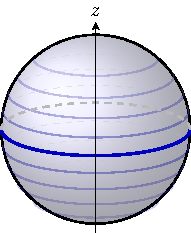
\includegraphics[width=.9\textwidth]{convert/integral-ball}            
          \end{center}
        \end{column}
    \end{columns}
\end{frame}

\begin{frame}
    \frametitle<presentation>{Das Volumen der Einheitskugel}
    \begin{itemize}
        \item Betrachten wir den Schnitt der Kugel mit der $xz$-Ebene, so sehen wir, dass $r(z)=\sqrt{1-z^2}$
        \item Integral über die Kreisflächen
        \begin{gather*}
            V = \int_{-1}^1 A\bigl(r(z)\bigr)\,dz
            = \int_{-1}^1 A\Bigl(\sqrt{1-z^2}\Bigr)\,dz
            = \pi \int_{-1}^1 \bigl(1-z^2\bigr)\,dz
        \end{gather*}
        \item Einsetzen der Stammfunktionen ergibt
        \begin{gather*}
            \int_{-1}^1 \bigl(1-z^2\bigr)\,dz
            = \left[ z-\frac{z^3}3\right]_{-1}^1
            = \left(1-\frac13\right) - \left(-1 - \frac13\right)
            = \frac43
        \end{gather*}
        \item Wir erhalten das Volumen
        \begin{gather*}
            V = \frac43\pi
        \end{gather*}
    \end{itemize}
\end{frame}

\begin{Aufgabe}
    Berechnen Sie das Volumen $V(r)$ einer Kugel vom Radius $r$.
\end{Aufgabe}

\begin{frame}{Berechnung von Volumina}
    Aus der Berechnung des Kugelvolumens können wir ein allgemeines Prinzip der Berechnung von Volumina ableiten:

    \begin{enumerate}
        \item Wir wählen eine \glqq{}Achse\grqq{} im Raum
        \item Wir bestimmen für jeden Punkt der Achse die Fläche des Schnitts in der Ebene senkrecht zu dieser Achse
        \begin{itemize}
            \item Eventuell ist hier auch Integration nötig
        \end{itemize}
        \item Wir integrieren diese Flächen entlang der Achse
    \end{enumerate}
\end{frame}

\begin{Aufgabe}
    Berechnen Sie das Volumen des Rotationskörpers (schlagen Sie den Begriff ggf.\ nach), der auf der $z$-Achse zwischen $-\pi/2$ und $\pi/2$ liegt und dessen Radius
    \begin{gather*}
        r(z) = \cos z
    \end{gather*}
    ist.
\end{Aufgabe}

\begin{Aufgabe}
    \begin{minipage}[b]{.64\textwidth}
      Ein geschraubter Zylinder habe folgende Maße:
      \begin{gather*}
          z\in[0,2\pi]
      \end{gather*}
    und auf Höhe $z$ sei sein Querschnitt ein Quadrat, dessen Eckpunkte die Koordinaten
      \begin{gather*}
          \begin{pmatrix}
          \cos z\\\sin z
          \end{pmatrix},\;
          \begin{pmatrix}
          -\sin z\\\cos z
          \end{pmatrix},\;
          \begin{pmatrix}
          -\cos z\\ -\sin z
          \end{pmatrix},\;
          \begin{pmatrix}
          \sin z\\-\cos z
          \end{pmatrix}
      \end{gather*}
      haben. Berechnen Sie sein Volumen!
    \end{minipage}
    \begin{minipage}[b]{.35\textwidth}
    \begin{center}
    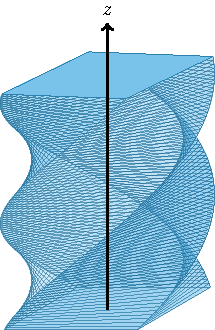
\includegraphics[width=.9\textwidth]{convert/integral-helix}
    \end{center}
    \end{minipage}
\end{Aufgabe}

\mode<all>
